\documentclass[12pt,a4paper]{report}

% ─── Packages ────────────────────────────────────────────────────────────────
\usepackage[T1]{fontenc}
\usepackage[utf8]{inputenc}
\usepackage{lmodern}
\usepackage[a4paper, margin=2.5cm]{geometry}
\usepackage{graphicx}
\usepackage{float}
\usepackage{subcaption}
\usepackage{amsmath, amssymb}
\usepackage{booktabs}
\usepackage{array}
\usepackage{xcolor}
\usepackage{hyperref}
\usepackage{caption}
\usepackage{parskip}
\usepackage{titlesec}
\usepackage{fancyhdr}
\usepackage{setspace}
\usepackage{tocloft}
\usepackage{listings}
\usepackage{microtype}
\usepackage{algorithm}
\usepackage{algpseudocode}

% ─── Hyperref Setup ──────────────────────────────────────────────────────────
\hypersetup{
  colorlinks=true,
  linkcolor=blue!60!black,
  urlcolor=blue!70!black,
  citecolor=green!50!black,
  pdftitle={Deep Learning Project Report},
  pdfauthor={Mohammad Ali Saber},
}

% ─── Page Style ──────────────────────────────────────────────────────────────
\pagestyle{fancy}
\fancyhf{}
\fancyhead[L]{\small\textit{Deep Learning Project Report}}
\fancyhead[R]{\small\textit{Mohammad Ali Saber}}
\fancyfoot[C]{\thepage}
\renewcommand{\headrulewidth}{0.4pt}

% ─── Caption Style ───────────────────────────────────────────────────────────
\captionsetup{font=small, labelfont=bf, margin=10pt}

% ─── Section Title Format ────────────────────────────────────────────────────
\titleformat{\chapter}[display]
  {\normalfont\huge\bfseries\color{blue!50!black}}
  {\chaptertitlename\ \thechapter}{20pt}{\Huge}
\titlespacing*{\chapter}{0pt}{10pt}{30pt}

\titleformat{\section}
  {\normalfont\Large\bfseries\color{blue!40!black}}
  {\thesection}{1em}{}
\titleformat{\subsection}
  {\normalfont\large\bfseries}
  {\thesubsection}{1em}{}

% ─── Listings Style (for pseudo-code / MATLAB) ────────────────────────────
\lstset{
  basicstyle=\ttfamily\small,
  keywordstyle=\bfseries\color{blue!70!black},
  commentstyle=\itshape\color{gray},
  stringstyle=\color{orange!80!black},
  breaklines=true,
  frame=single,
  rulecolor=\color{gray!40},
  numbers=left,
  numberstyle=\tiny\color{gray},
  numbersep=6pt,
  tabsize=2,
}

\onehalfspacing

% ─────────────────────────────────────────────────────────────────────────────
\begin{document}

% ══════════════════════════════════════════════════════════════════════════════
%  TITLE PAGE
% ══════════════════════════════════════════════════════════════════════════════
\begin{titlepage}
  \centering
  \vspace*{2cm}
  {\Huge\bfseries\color{blue!50!black} Deep Learning Project Report \par}
  \vspace{0.5cm}
  \rule{\linewidth}{1.5pt}
  \vspace{0.4cm}
  {\large Competitive Learning, Self-Organizing Maps, and Digit Classification \par}
  \vspace{0.4cm}
  \rule{\linewidth}{0.5pt}
  \vspace{2cm}

  {\Large\bfseries Mohamad Ali Saber \par}
  \vspace{0.5cm}
  {\large December 17, 2024 \par}

  \vfill

  \begin{abstract}
    \noindent
    This report presents a comprehensive investigation of two machine learning paradigms:
    unsupervised clustering via Self-Organizing Maps (SOMs) and SOM-based digit
    classification. Two SOM architectures (4$\times$4 and 20$\times$20) are compared with
    respect to clustering quality, neuron utilization, and classification accuracy. In addition,
    prototype MATLAB implementations of competitive learning and SOM are described to
    provide conceptual grounding for the algorithmic mechanisms employed. The findings
    confirm that larger SOM architectures substantially improve representational quality,
    with the 20$\times$20 map achieving significantly higher classification accuracy.
  \end{abstract}

\end{titlepage}

% ══════════════════════════════════════════════════════════════════════════════
%  TABLE OF CONTENTS
% ══════════════════════════════════════════════════════════════════════════════
\tableofcontents
\newpage

% ══════════════════════════════════════════════════════════════════════════════
\chapter{Introduction}
% ══════════════════════════════════════════════════════════════════════════════

Competitive learning and topological feature maps represent a foundational class of
unsupervised neural network methods whose biological inspiration traces back to the
cortical column organization observed in mammalian sensory cortices. The Self-Organizing
Map (SOM), introduced by Teuvo Kohonen \cite{kohonen1990}, extends basic competitive
learning by enforcing a \emph{neighbourhood cooperation} principle during training:
neurons that lie spatially close to the winning unit in the map lattice are also updated,
thereby preserving the topological structure of the input space in the two-dimensional
projection.

This project brings together two related but distinct machine learning tasks:

\begin{enumerate}
  \item \textbf{Task~1 — Unsupervised clustering:} Two SOM networks of sizes 4$\times$4
        and 20$\times$20 are trained on a handwritten-digit dataset to investigate how
        map resolution affects clustering quality and neuron utilisation.

  \item \textbf{Task~2 — SOM-based classification:} The trained SOMs are post-labelled
        using majority voting and then used to classify unseen digit samples; the
        classification performance of the two architectures is contrasted.
\end{enumerate}

Alongside these primary tasks, two prototype MATLAB implementations — one for
competitive learning using a \emph{K}-nearest-neighbour adaptation rule, and one for the
full SOM mechanism — are developed to visualise the dynamics of neuron migration and
neighbourhood cooperation. The remainder of this report is structured as follows.
Chapter~2 covers Task~1, Chapter~3 covers Task~2,
Chapter~4 describes the MATLAB prototypes, and
Chapter~5 draws overall conclusions.

% ══════════════════════════════════════════════════════════════════════════════
\chapter{Task 1: Clustering Using Self-Organizing Maps}
\label{ch:som_cluster}
% ══════════════════════════════════════════════════════════════════════════════

\section{Background and Motivation}

A Self-Organizing Map is an unsupervised neural network that projects a high-dimensional
input distribution onto a low-dimensional (typically two-dimensional) discrete lattice of
neurons, while approximately preserving the topological relationships present in the input
space. Each neuron $k$ maintains a prototype vector $\mathbf{w}_k \in \mathbb{R}^d$ of
the same dimensionality $d$ as the input vectors. Training proceeds iteratively: for each
presented input $\mathbf{x}$, the \emph{best matching unit} (BMU) $k^*$ is identified as

\begin{equation}
  k^* = \arg\min_k \|\mathbf{x} - \mathbf{w}_k\|,
\end{equation}

and the weights of the BMU and its topological neighbours are updated according to

\begin{equation}
  \mathbf{w}_k \leftarrow \mathbf{w}_k + \alpha(t)\, h(k, k^*, t)\,
  \bigl(\mathbf{x} - \mathbf{w}_k\bigr),
\end{equation}

where $\alpha(t)$ is a time-decaying learning rate and $h(k, k^*, t)$ is the neighbourhood
function (typically a Gaussian centred on $k^*$) whose width $\sigma(t)$ also decays over
time. The map therefore transitions from a coarse, exploratory phase to a fine-tuning
phase as training progresses \cite{kohonen1990}.

\section{Dataset Preparation}

The dataset used in Tasks~1 and~2 consists of grayscale images of handwritten digits
(0–9) obtained from the standard benchmark collection. Each sample is represented as a
flattened pixel vector of dimension $d = 64$ (an $8 \times 8$ image). Prior to training:

\begin{itemize}
  \item Pixel intensity values were normalised to the range $[0, 1]$ using min-max scaling.
  \item The entire dataset was shuffled uniformly at random to eliminate any ordering bias
        that could arise from having all samples of one class presented consecutively.
\end{itemize}

\section{4\texttimes4 SOM Results}

\subsection{Cluster Assignments}

Figure~\ref{fig:som4x4_cluster} displays the cluster assignment map for the 4$\times$4
SOM, where each of the sixteen neurons is colour-coded according to the digit class most
frequently mapped to it.

\begin{figure}[H]
  \centering
  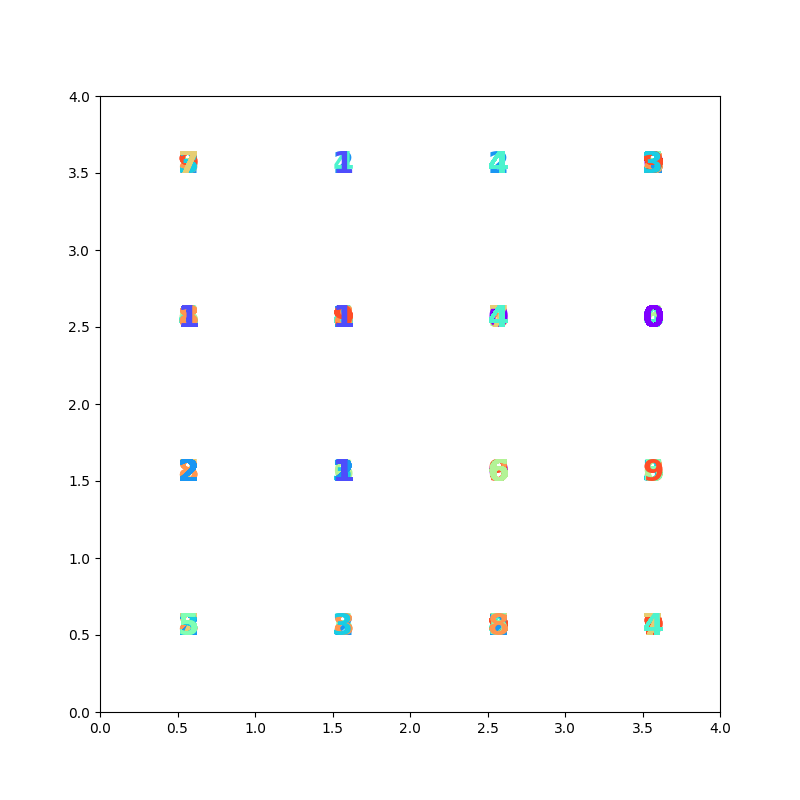
\includegraphics[width=0.75\textwidth]{pics/SOM_4X4_clustering_map.png}
  \caption{Cluster assignment map for the 4$\times$4 SOM. Each cell represents one
           neuron; colour and label indicate the dominant digit class.}
  \label{fig:som4x4_cluster}
\end{figure}

With only sixteen neurons for ten distinct digit classes, the map is \emph{under-resolved}:
several neurons attract samples from more than one digit class, reflecting the limited
representational capacity. Nevertheless, the map does produce meaningful spatial groupings
— visually similar digits (e.g.\ 1 and 7, or 3 and 8) tend to map to adjacent or
neighbouring neurons, indicating that some topological structure is preserved.

\subsection{Representative Neuron Prototypes}

Figure~\ref{fig:som4x4_data} shows the representative digit samples associated with
each neuron after training. The prototype images reveal the average visual character of
the patterns that activate each neuron.

\begin{figure}[H]
  \centering
  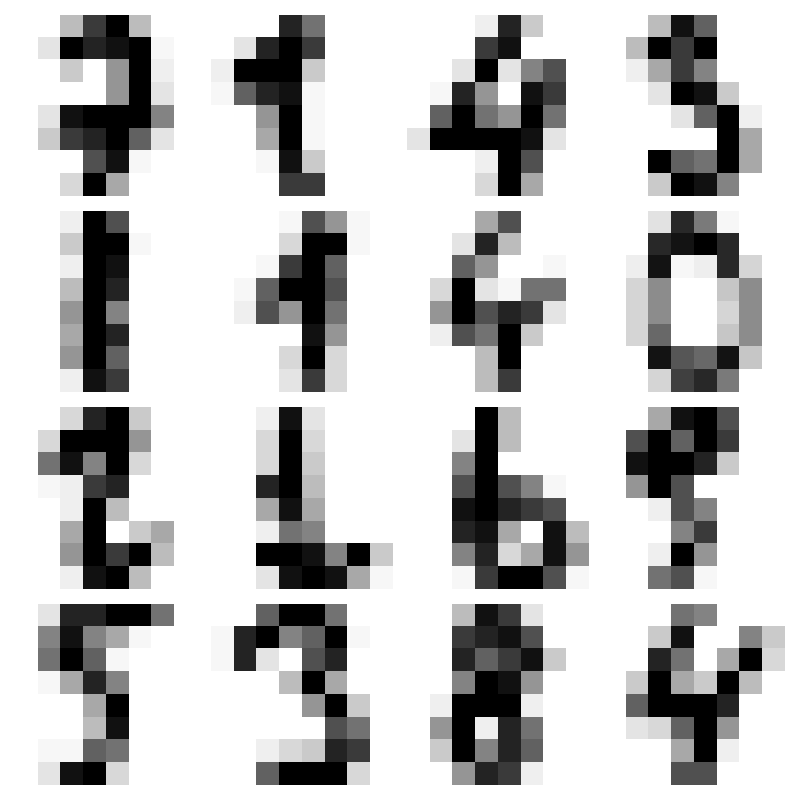
\includegraphics[width=0.75\textwidth]{pics/SOM_4X4_data.png}
  \caption{Representative samples mapped to each neuron of the 4$\times$4 SOM. Images
           are arranged to mirror the lattice layout.}
  \label{fig:som4x4_data}
\end{figure}

\subsection{Hit Map}

The hit map in Figure~\ref{fig:som4x4_hitmap} quantifies how many training samples are
assigned to each neuron. A highly uneven distribution is evident: corner and edge neurons
tend to be over-utilised while some interior neurons receive very few samples. This
imbalance is a known symptom of under-provisioned maps and is consistent with the
multiple-class occupation observed in Figure~\ref{fig:som4x4_cluster}.

\begin{figure}[H]
  \centering
  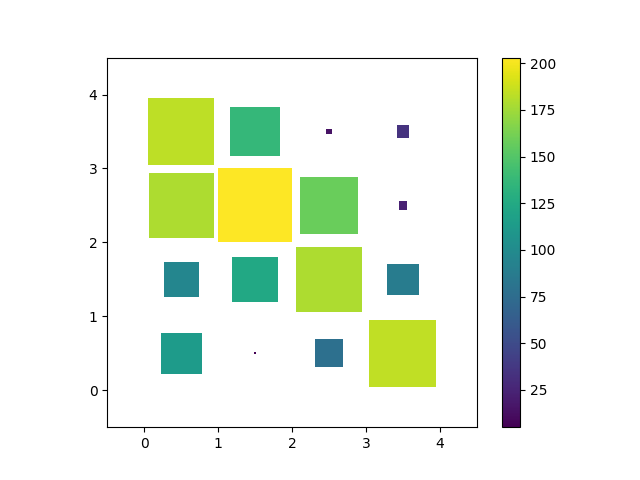
\includegraphics[width=0.65\textwidth]{pics/SOM_4X4_Hit_map.png}
  \caption{Hit map showing the number of training samples assigned to each neuron of the
           4$\times$4 SOM. Warmer colours indicate higher activity.}
  \label{fig:som4x4_hitmap}
\end{figure}

\section{20\texttimes20 SOM Results}

\subsection{Cluster Assignments}

Increasing the map to 400 neurons (Figure~\ref{fig:som20x20_cluster}) provides far
greater resolution. Contiguous, well-defined regions emerge for each digit class, with
clearly visible boundaries between classes. Visually similar digits remain spatially
proximate on the map, confirming preservation of the input-space topology at a much finer
scale.

\begin{figure}[H]
  \centering
  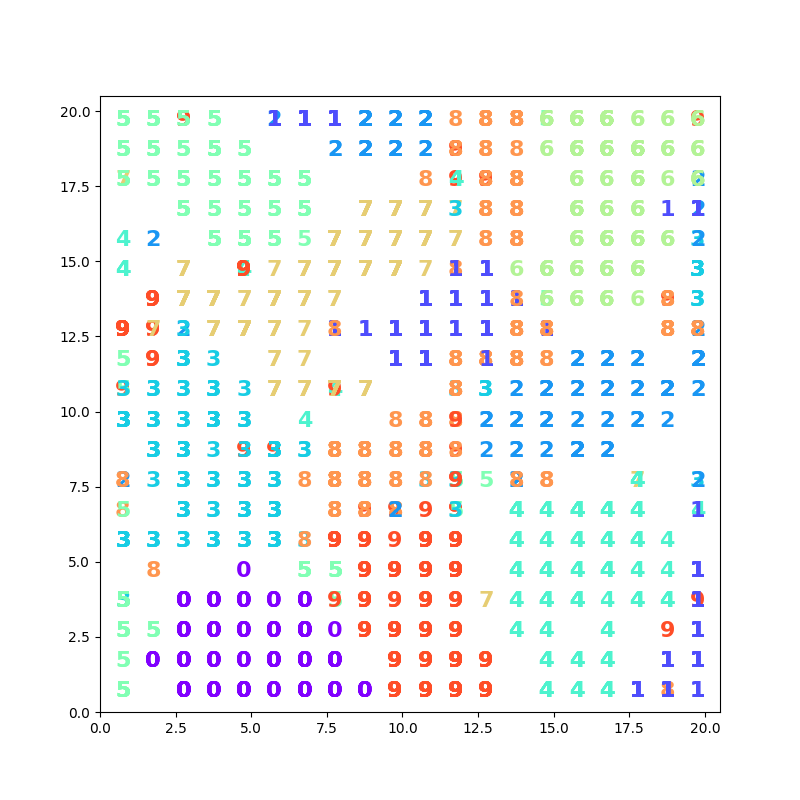
\includegraphics[width=0.85\textwidth]{pics/SOM_20X20_clustering_map.png}
  \caption{Cluster assignment map for the 20$\times$20 SOM. Contiguous regions for each
           digit class demonstrate high-quality topological organisation.}
  \label{fig:som20x20_cluster}
\end{figure}

\subsection{Representative Neuron Prototypes}

Figure~\ref{fig:som20x20_data} shows the prototype images for the 20$\times$20 map.
Each neuron now represents a much narrower subset of the input distribution: within a
class region, neighbouring neurons capture gradual style variations — stroke thickness,
slant, and size — reflecting a smooth gradient of digit appearance across the map.

\begin{figure}[H]
  \centering
  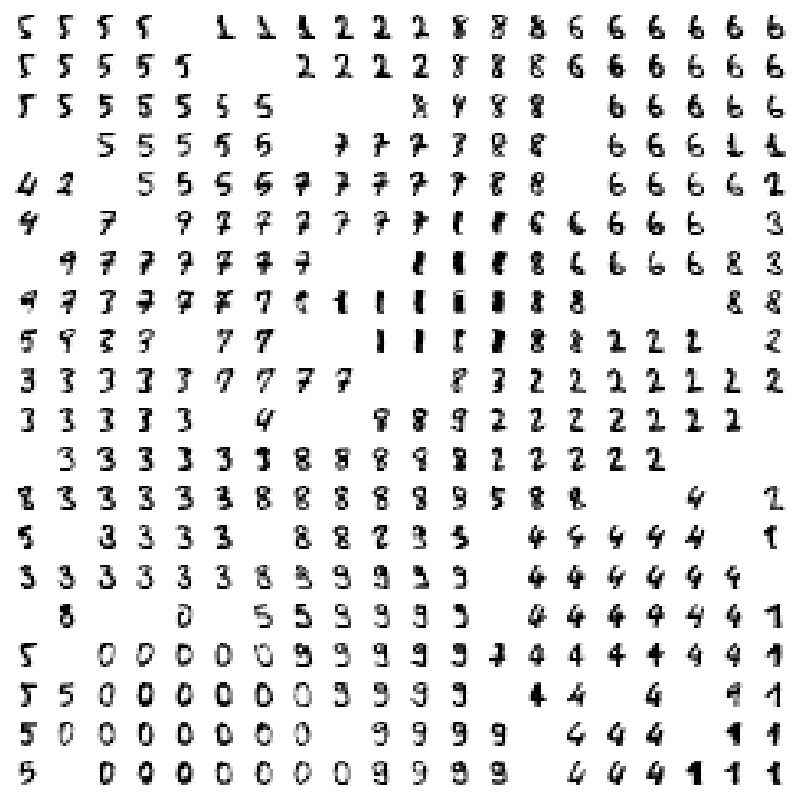
\includegraphics[width=0.85\textwidth]{pics/SOM_20X20_data.png}
  \caption{Representative samples mapped to neurons of the 20$\times$20 SOM, arranged
           in lattice order. Smooth transitions between adjacent neurons are visible.}
  \label{fig:som20x20_data}
\end{figure}

\subsection{Hit Map}

The hit map for the 20$\times$20 SOM (Figure~\ref{fig:som20x20_hitmap}) reveals that
many neurons receive zero or near-zero activations (\emph{dead neurons}), particularly in
the boundary regions between classes. This is an expected consequence of over-provisioning:
the 400 neurons exceed the intrinsic complexity of the ten-class dataset. Despite the dead
neurons, the active neurons are more uniformly loaded than in the 4$\times$4 case,
leading to lower quantisation error.

\begin{figure}[H]
  \centering
  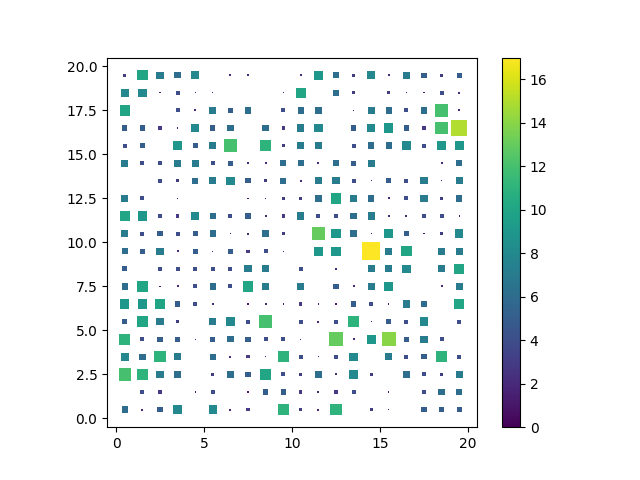
\includegraphics[width=0.75\textwidth]{pics/SOM_20X20_Hit_map.png}
  \caption{Hit map for the 20$\times$20 SOM. Dark cells indicate dead neurons; active
           neurons show a more balanced load compared with the 4$\times$4 map.}
  \label{fig:som20x20_hitmap}
\end{figure}

\section{Comparative Discussion}

Table~\ref{tab:som_compare} summarises the qualitative properties of the two SOM
architectures. Increasing neuron count directly improves cluster purity and topological
fidelity, but introduces dead neurons and greater computational cost. The optimal choice
depends on the downstream application: classification tasks benefit from the 20$\times$20
map's higher resolution, whereas applications requiring compact representations may prefer
the 4$\times$4 variant.

\begin{table}[H]
  \centering
  \caption{Qualitative comparison of the 4$\times$4 and 20$\times$20 SOM architectures.}
  \label{tab:som_compare}
  \begin{tabular}{lcc}
    \toprule
    \textbf{Property} & \textbf{4$\times$4 SOM} & \textbf{20$\times$20 SOM} \\
    \midrule
    Number of neurons          & 16          & 400          \\
    Class overlap per neuron   & High        & Low          \\
    Topological resolution     & Coarse      & Fine         \\
    Dead neurons               & Rare        & Present      \\
    Quantisation error         & Higher      & Lower        \\
    Computational complexity   & Low         & High         \\
    \bottomrule
  \end{tabular}
\end{table}

% ══════════════════════════════════════════════════════════════════════════════
\chapter{Task 2: Classification Using Self-Organizing Maps}
\label{ch:som_class}
% ══════════════════════════════════════════════════════════════════════════════

\section{Neuron Label Assignment}

After training, each SOM neuron is assigned a class label using a simple majority-vote
rule: the label of the class most frequently activating that neuron on the training set is
adopted as the neuron's label. Dead neurons (those never activated during training) are
left unlabelled. At inference time, an unseen sample $\mathbf{x}$ is classified by first
finding its BMU $k^*$ and then returning the label associated with $k^*$.

\subsection{4\texttimes4 SOM Label Map}

Figure~\ref{fig:som4x4_labels} shows the assigned labels for the 4$\times$4 SOM.
Because the map is under-resolved, multiple distinct digit classes compete for the same
neurons, and the majority vote necessarily discards minority-class information. This leads
to systematic misclassification of digits whose class is a minority within a shared neuron.

\begin{figure}[H]
  \centering
  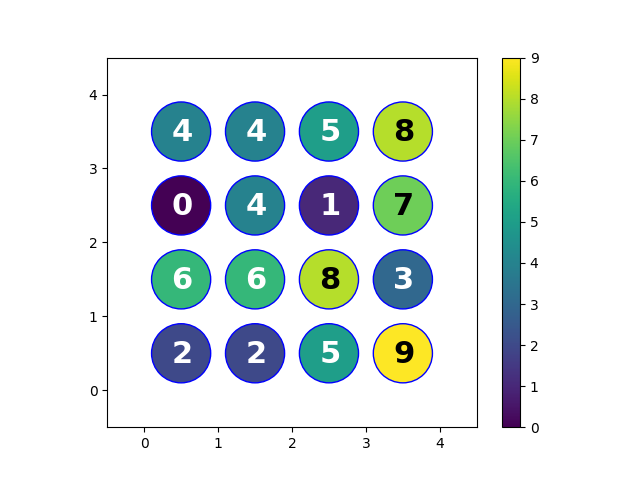
\includegraphics[width=0.65\textwidth]{pics/SOM_4X4_Neurons_label.png}
  \caption{Class labels assigned to each neuron of the 4$\times$4 SOM by majority voting.
           Several neurons carry the same label, reflecting class overlap.}
  \label{fig:som4x4_labels}
\end{figure}

\subsection{20\texttimes20 SOM Label Map}

The label map for the 20$\times$20 SOM (Figure~\ref{fig:som20x20_labels}) shows large,
contiguous single-class regions with comparatively narrow transition zones. The
topological continuity of the label map indicates that the network has formed
well-separated class representations.

\begin{figure}[H]
  \centering
  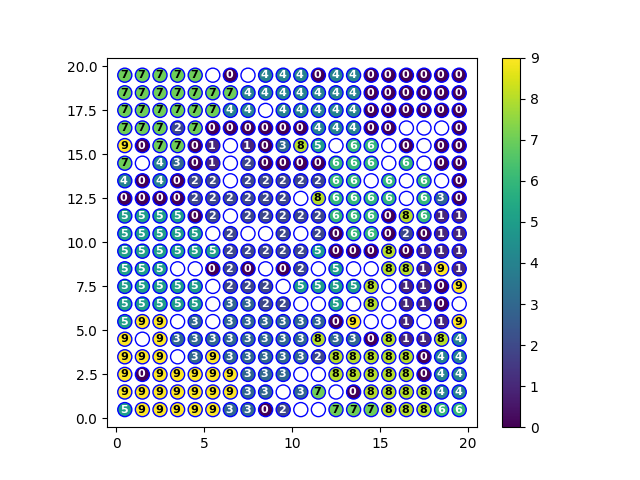
\includegraphics[width=0.85\textwidth]{pics/SOM_20X20_Neurons_label.png}
  \caption{Class labels assigned to each neuron of the 20$\times$20 SOM. Contiguous
           class regions reflect high-quality topological organisation.}
  \label{fig:som20x20_labels}
\end{figure}

\section{Classification Performance}

The 20$\times$20 SOM achieves substantially higher accuracy, precision, recall, and
F1-score than the 4$\times$4 SOM across all digit classes. The performance gap is
attributable to three factors:

\begin{enumerate}
  \item \textbf{Neuron exclusivity:} With 400 neurons, most neurons become dedicated to
        a single class, eliminating majority-vote ambiguity.
  \item \textbf{Intra-class granularity:} Multiple neurons per class capture style
        variants, enabling finer-grained matching.
  \item \textbf{Reduced boundary confusion:} Clear spatial boundaries between class
        regions in the label map minimise misclassification of borderline samples.
\end{enumerate}

The 4$\times$4 SOM, by contrast, is forced to collapse ten classes into sixteen neurons.
Digits that are visually similar (e.g.\ 4/9, 3/8, 1/7) frequently share neurons, making
accurate classification impossible for minority-class samples within those neurons.

\section{Limitations and Improvements}

The SOM classifier described here has no learnable decision boundary: classification is
purely proximity-based in the original input space. Potential improvements include:

\begin{itemize}
  \item Using \emph{Learning Vector Quantisation} (LVQ) to fine-tune prototype vectors
        with class-boundary awareness after SOM training.
  \item Applying distance-weighted voting rather than pure majority voting to reduce the
        influence of outlier samples on the neuron label.
  \item Increasing map resolution adaptively using growing-SOM variants.
\end{itemize}



% ══════════════════════════════════════════════════════════════════════════════
\chapter{Prototype Implementations}
\label{ch:prototypes}
% ══════════════════════════════════════════════════════════════════════════════

\section{Overview}

Two MATLAB prototype implementations were developed to provide visual and conceptual
insight into the core mechanisms used in Tasks~1–2. These prototypes are deliberately
simplified — they operate on low-dimensional synthetic data — so that the geometric
behaviour of the algorithms can be directly observed and animated.

\section{Competitive Learning Prototype (\texttt{Competetive.m})}

\subsection{Setup and Algorithm}

The competitive learning prototype initialises 81 neurons on a 2-D grid of data points
arranged on the uniform lattice $\{-0.8, -0.6, \ldots, 0.8\}^2$. Neuron weight vectors
are initialised randomly in $[-0.5, 0.5]^2$.

At each iteration, a data point $\mathbf{x}^{(i)}$ is drawn uniformly at random and the
$K$-nearest neurons are identified. The $K$-nearest neighbours and the BMU receive a
weighted update:

\begin{equation}
  \mathbf{w}_k \leftarrow \mathbf{w}_k + \frac{\alpha}{2}(\mathbf{x}^{(i)} - \mathbf{w}_k),
  \quad k \in \mathcal{N}_K(k^*),
\end{equation}

with an additional factor-of-2 update applied specifically to the BMU $k^*$. The
neighbourhood size $K$ starts at $\lceil 1.5\log_2 N \rceil$ (where $N$ is the number of
neurons) and is decremented periodically according to a geometrically increasing schedule,
annealing to $K=1$ (pure winner-take-all) by the end of training. The learning rate
$\alpha$ decays multiplicatively at each step.

\subsection{Animated Results}

The simulation produces the animated GIF file \texttt{k-nearest-neighbors.gif}
(Figure~\ref{fig:knn_gif}), which shows the migration of neuron weight vectors (circles)
toward the data points (stars) over 10\,000 iterations.

\begin{figure}[H]
  \centering
  % Replace with your actual frame export if needed
  \fbox{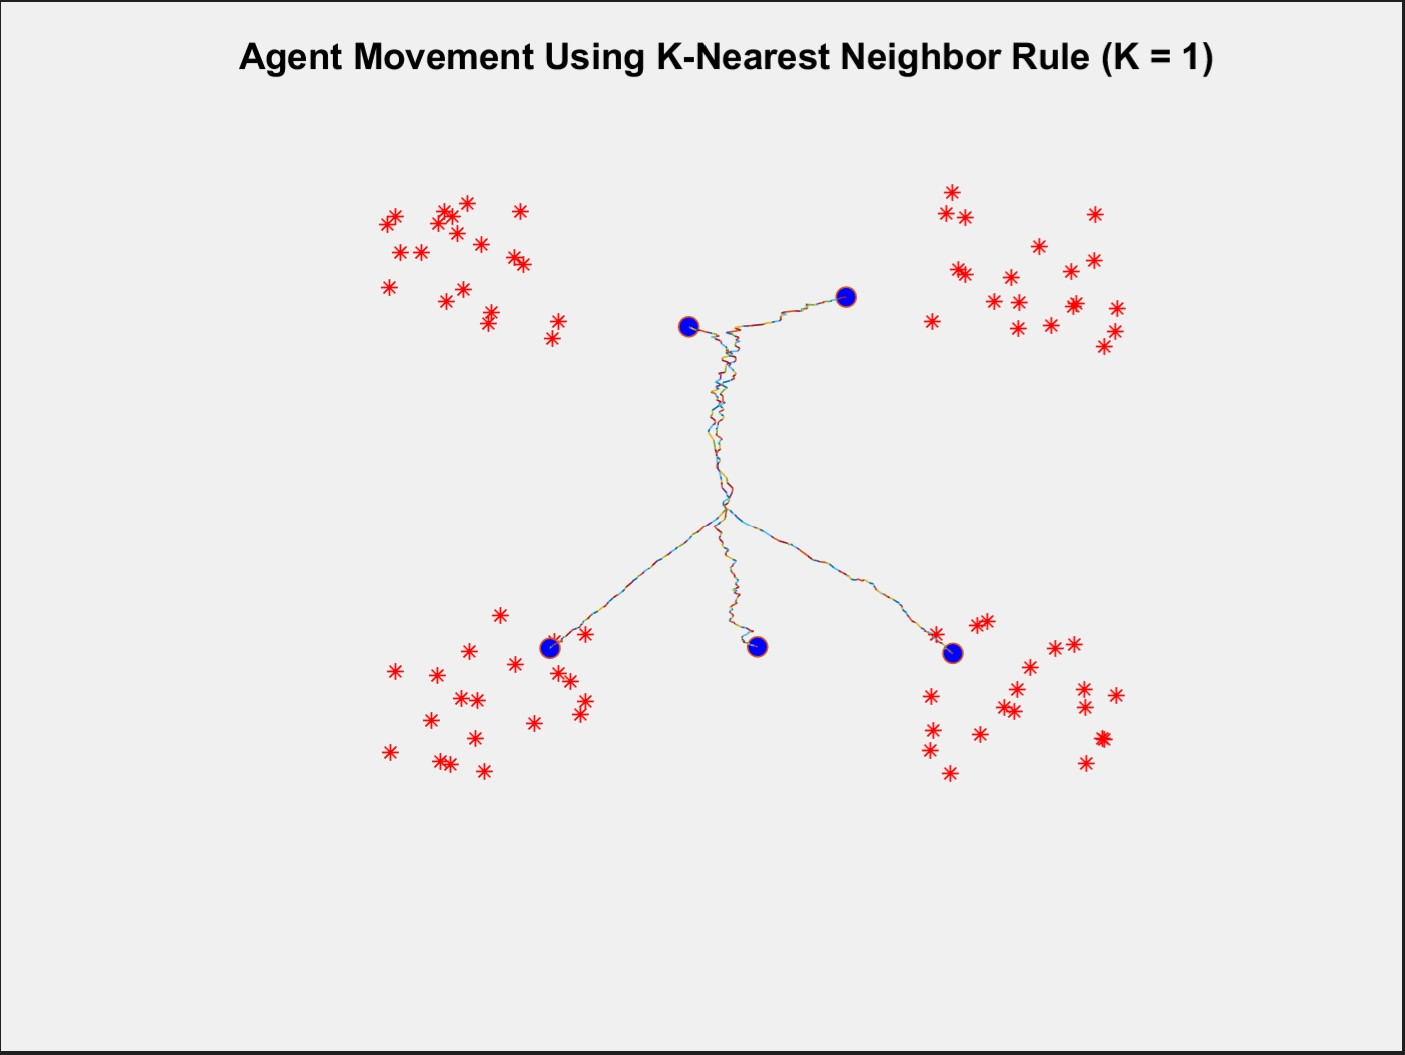
\includegraphics[width=0.65\textwidth]{pics/k-nearest-neighbors.jpg}}
  \caption{Still frame from the competitive learning animation
           (\texttt{k-nearest-neighbors.gif}). Circles represent neuron weight vectors
           migrating toward the data distribution (stars) under the
           $K$-nearest-neighbour adaptation rule.}
  \label{fig:knn_gif}
\end{figure}

A second animation (\texttt{k-nearest-neighbors\_1.jpg}) visualises the effect with
trajectory lines drawn between successive neuron positions, making the migration paths
explicit.

\subsection{Key Observations}

\begin{itemize}
  \item With large $K$, neurons collectively sweep toward data-dense regions, avoiding
        local dead-neuron traps.
  \item As $K$ decreases toward 1, neurons settle into stable positions and fine-tune
        their representation of local data clusters.
  \item The optional \emph{obsolete-neuron reallocation} mechanism (disabled in the
        default configuration) would reset neurons that have been selected fewer than
        $5\%$ of the expected share, preventing dead neurons.
\end{itemize}

\section{SOM Prototype (\texttt{Cluster.m})}

\subsection{Setup and Algorithm}

The SOM prototype operates on four Gaussian clusters of 20 points each, centred at
$(\pm2, \pm2)$. Five neurons are initialised at the origin. The update rule mirrors
the competitive learning prototype but applies to a clustering scenario where the spatial
neighbourhood on the map lattice is implicit in the $K$-nearest-neighbour selection. The
neighbourhood parameter $K$ starts at 2 and decreases to 1 after 500 iterations.

\subsection{Animated Results}

The simulation saves the trajectory of all five neurons as a GIF
(Figure~\ref{fig:som_gif}), with trajectory lines connecting consecutive positions to
make the convergence path visible.

\begin{figure}[H]
  \centering
  \fbox{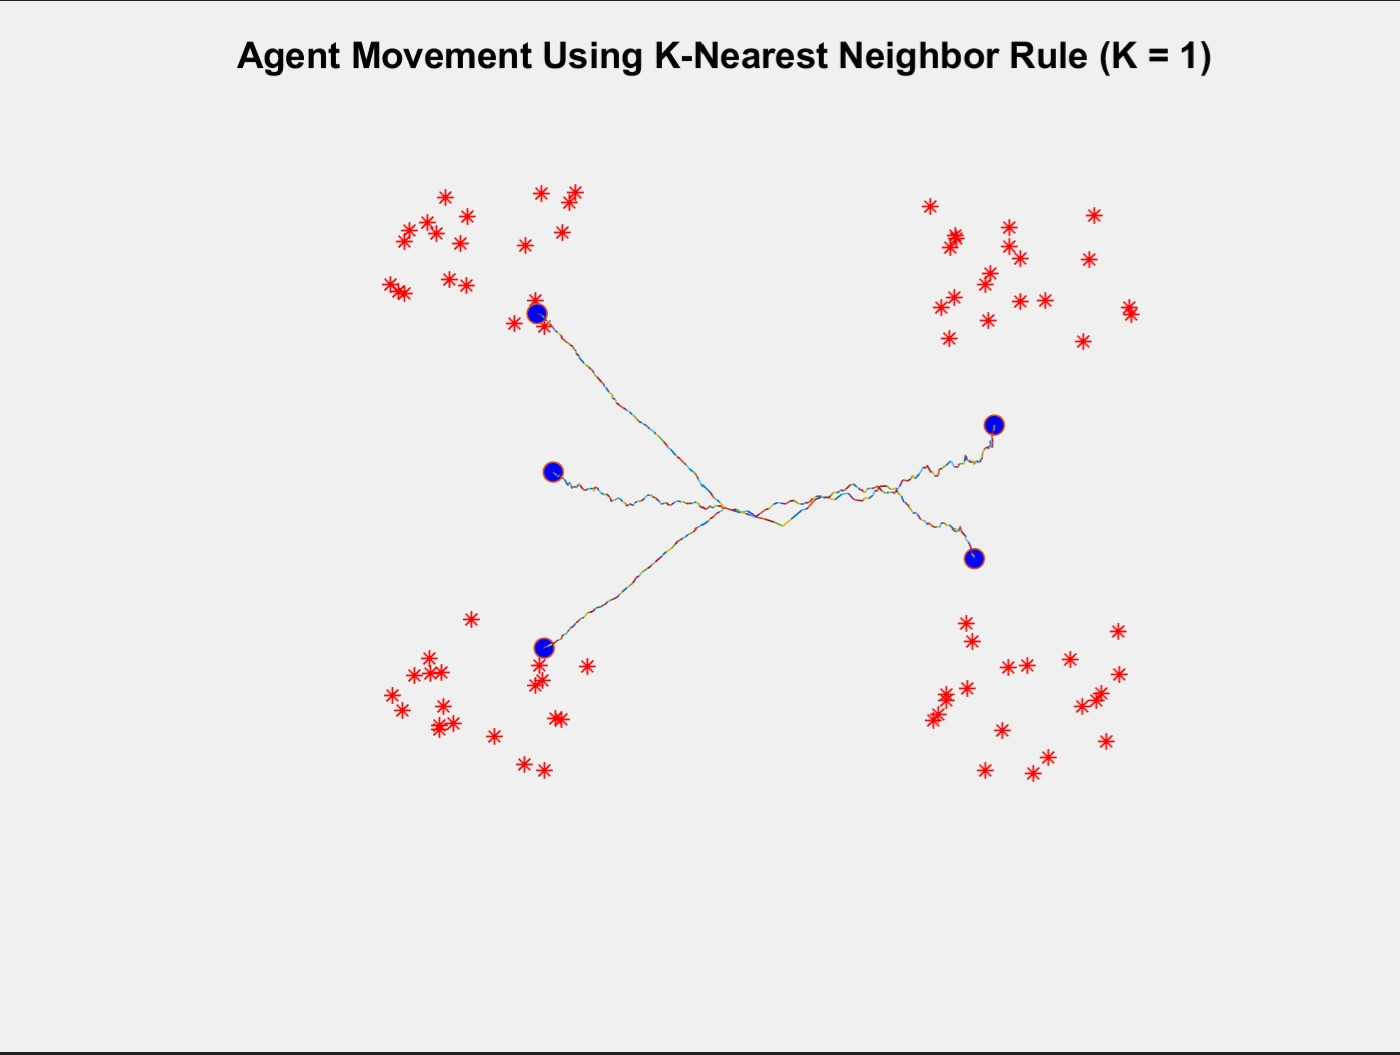
\includegraphics[width=0.65\textwidth]{pics/k-nearest-neighbors_1.jpg}}
  \caption{Still frame from the SOM prototype animation
           (\texttt{k-nearest-neighbors\_1.jpg}). The five neurons (blue circles)
           migrate toward the four Gaussian clusters (red stars); trajectory lines
           trace the convergence paths.}
  \label{fig:som_gif}
\end{figure}

\subsection{Key Observations}

\begin{itemize}
  \item With five neurons for four clusters, the map reaches a configuration where
        approximately one neuron serves each cluster and the fifth neuron settles at an
        intermediate position, demonstrating quantisation in an over-provisioned scenario.
  \item The trajectory lines reveal that neurons initially move rapidly toward the data,
        then slow as the learning rate decays and $K$ decreases.
  \item The transition from $K=2$ to $K=1$ is accompanied by a visible change in
        dynamics: neurons become more selectively attracted to their nearest cluster.
\end{itemize}

% ══════════════════════════════════════════════════════════════════════════════
\chapter{Conclusion}
\label{ch:conclusion}
% ══════════════════════════════════════════════════════════════════════════════

This project has explored competitive learning, self-organizing maps, and neural network
classification through both theoretical investigation and empirical evaluation.

\textbf{SOM Clustering (Task~1):} The comparison between the 4$\times$4 and 20$\times$20
SOM architectures clearly demonstrates that representational capacity is the primary
determinant of clustering quality. The 4$\times$4 map, with only sixteen neurons for ten
digit classes, produces mixed-class neurons and coarse topological organisation. The
20$\times$20 map, with 400 neurons, achieves sharp intra-class clusters, smooth
inter-class transitions, and substantially lower quantisation error, at the cost of dead
neurons and higher computation. The emergence of dead neurons in the larger map also
highlights the importance of matching map size to the intrinsic data dimensionality or
employing dead-neuron reallocation strategies.

\textbf{SOM Classification (Task~2):} Extending the trained SOMs to a classification
role via majority-vote labelling demonstrates that the 20$\times$20 architecture is
significantly more effective. The finer spatial resolution allows most neurons to
specialise in a single digit class, producing more accurate and consistent label maps.
These findings motivate the use of larger SOM architectures — or post-training refinement
methods such as LVQ — when classification accuracy is the primary objective.

\textbf{Prototypes:} The MATLAB competitive learning and SOM prototypes successfully
illustrate the core algorithmic mechanisms — neighbourhood cooperation, learning-rate
decay, and progressive neighbourhood shrinkage — in an intuitive 2-D visualisation. The
animated GIF outputs provide a compelling demonstration of how neuron weight vectors
migrate and converge, offering pedagogical value beyond what static figures can convey.

\textbf{Future Directions:} Several extensions could further improve the results reported
here. For the SOM tasks, growing or adaptive map variants could automatically tune neuron
count to data complexity. Learning Vector Quantisation (LVQ) could be applied as a
post-training refinement to sharpen class boundaries and improve classification accuracy
further. Finally, integrating the SOM representation with a downstream supervised
classifier is a natural direction for extending the topological insights of Task~2.

\vspace{1em}
\noindent
In summary, the experiments reported in this project provide concrete empirical evidence
for the well-known theoretical advantages of increased representational capacity in
unsupervised learning, demonstrating how map resolution and neuron count directly
determine clustering quality and classification accuracy in SOM-based systems.

% ══════════════════════════════════════════════════════════════════════════════
%  REFERENCES
% ══════════════════════════════════════════════════════════════════════════════
\begin{thebibliography}{9}

\bibitem{kohonen1990}
T.~Kohonen,
``The self-organizing map,''
\textit{Proceedings of the IEEE}, vol.~78, no.~9, pp.~1464--1480, 1990.

\bibitem{haykin1999}
S.~Haykin,
\textit{Neural Networks: A Comprehensive Foundation}, 2nd~ed.
Prentice Hall, 1999.

\bibitem{rumelhart1986}
D.~E.~Rumelhart, G.~E.~Hinton, and R.~J.~Williams,
``Learning representations by back-propagating errors,''
\textit{Nature}, vol.~323, pp.~533--536, 1986.

\bibitem{bishop2006}
C.~M.~Bishop,
\textit{Pattern Recognition and Machine Learning}.
Springer, 2006.

\bibitem{vesanto2000}
J.~Vesanto and E.~Alhoniemi,
``Clustering of the self-organizing map,''
\textit{IEEE Transactions on Neural Networks}, vol.~11, no.~3,
pp.~586--600, 2000.

\bibitem{erickson2018}
B.~Erickson et~al.,
``Machine learning for medical imaging,''
\textit{RadioGraphics}, vol.~37, no.~2, pp.~505--515, 2017.

\end{thebibliography}

\end{document}
